% !TEX encoding = UTF-8 Unicode 
%
% Use:
% magister / inzynier - for master thesis or engineering thesis
% druk / archiwum - for print version or archive version
% en - to translate template into english
% examples:
%\documentclass[inzynier,druk,en] - master thesis, print version, english
%\documentclass[magister,druk,en]{dyplom}
%\documentclass[magister,druk]{dyplom}

\documentclass[inzynier,druk]{dyplom}

\usepackage[utf8]{inputenc}
\usepackage{hyperref}

% Maximum section's depth.
\setcounter{secnumdepth}{4}

% Listings settings
% \setminted{breaklines, 
% frame=lines,           
% framesep=3mm,          
% baselinestretch=1.1,   
% fontsize=\small,       
% % linenos              % line numbering
% }

\usepackage{lipsum}
\usepackage{tabularx}
\usepackage{listings}
\usepackage{subcaption}

% \faculty{Faculty of \dots}                   % Uncomment if applicable
\fieldofstudy{Informatyka Techniczna (ITE)}                          
\author{Józef Bossowski}
\title{Projekt i implementacja wieloosobowej gry on-line z użyciem silnika Godot}
\supervisor{Dr inż. Tomasz Walkowiak}
% \consultant{Consultant's name}               % Uncomment if applicable
\specialisation{IGM}                         % Uncomment if applicable
\keywords{Godot, gra sieciowa}	% 3-5 keywords  

\begin{document}

\maketitle

\abstract{
Celem niniejszej pracy dyplomowej było zaprojektowanie i stworzenie wieloosobowej gry sieciowej. Gra miała zostać stworzona z wykorzystaniem silnika Godot. Gra wykorzystuje grafikę 3D oraz widok trzecioosobowy. Aplikacja umożliwia połączenie od dwóch do sześciu graczy w sieci lokalnej LAN. Stworzona aplikacja została przetestowana jednostkowo i integracyjnie z wykorzystaniem narzędzia GUT oraz manualnie pod systemem operacyjnym Windows 10.  

Przed rozpoczęciem implementacji przygotowana została koncepcja gry, plan mechanik oraz najważniejszych systemów. W następnej kolejności stworzony został prototyp. Przygotowując prototyp przeprowadzona została analiza trudności implementacji systemu sieciowego. 

Zaprojektowane zostały interfejsy użytkownika oraz najważniejsze podsystemy. W następnej kolejności zostały one zaimplementowane zgodnie z koncepcją i projektami. Została również przeprowadzona dyskusja wyników, analiza wniosków. Opisano również możliwości dalszego rozwoju projektu.
}{
The goal of this thesis was to design and create a game featuring an on-line multiplayer using the Godot game engine. The game uses 3D graphics, providing player with third person view. Application enables two to six players to connect over local network. Unit and integration tests were created using the GUT toolkit. Manual tests were also ran under Windows 10.

Before implementing the software, a game design concept was formulated. It consists of plans for mechanics and systems to be featured in the game. A prototype was created in order to analyze the difficulty of implementing the network system. 

Designs included graphical interfaces and the most important subsystems. Those were implemented according to concepts and designs. Finally, the results were analyzed and some ways of improving the project in the future were proposed.
}

\tableofcontents

% \chapter*{Wst�p}
\section{Cel pracy}

Celem niniejszej pracy dyplomowej jest zaprojektowanie oraz zaprogramowanie sieciowej gry wieloosobowej.

Gra b�dzie umo�liwia� po��czenie od dw�ch do sze�ciu os�b w sieci lokalnej. Aplikacja zostanie przygotowana na komputery PC z systemem Windows 10. 
Serwerem gry b�dzie komputer jednego z graczy, nazywanego r�wnie� \emph{hostem}.
Zar�wno mechaniki gry jak i system sieciowy zostan� zaimplementowane z wykorzystaniem silnika Godot. (cite: godot page)
W celu zapewnienia p�ynnej i komfortowej rozgrywki zostan� zastosowane techniki predykcji klienta.

Pocz�tkowo przygotowane zostan�:
\begin{itemize}
    \item \emph{Koncepcja gry} - projekt mechanik gry, projekt wizualny, elementy \emph{game designu};
    \item \emph{Projekt aplikacji} - projekt interfejsu u�ytkownika, plan przygotowania systemu sieciowego oraz dzia�anie mechanik;
    \item \emph{Prototyp aplikacji} - pocz�tkowa, okrojona wersja gry, przygotowana w celu zapoznania si� z dzia�aniem silnika oraz w celu okre�lenia potencjalnych problem�w z p�niejsz� implementacj�. 
\end{itemize}

Powy�sze elementy b�d� przygotowywane r�wnolegle, aby wiedza pozyskana w czasie rozwijania jednego mog�a mo�liwie najlepiej wesprze� pozosta�e.

\section{Technologie}
W rozwoju projektu wykorzystane zostan� poni�sze technologie:
\begin{itemize}
    \item \emph{Godot} - Silnik gier; implementacja mechanik gry, silnik fizyczny, komunikacja sieciowa, wysokopoziomowy interfejs sieciowy;
    \item \emph{Git}, \emph{GitHub} - System kontroli wersji;
    \item \emph{Blender} - Modelowanie 3D, przygotowanie materia��w;
    \item \emph{Trello} - Planowanie, harmonogram pracy;
\end{itemize}

\chapter*{Wst�p}
\section{Cel pracy}

Celem niniejszej pracy dyplomowej jest zaprojektowanie oraz zaprogramowanie sieciowej gry wieloosobowej.

Gra b�dzie umo�liwia� po��czenie od dw�ch do sze�ciu os�b w sieci lokalnej. Aplikacja zostanie przygotowana na komputery PC z systemem Windows 10. 
Serwerem gry b�dzie komputer jednego z graczy, nazywanego r�wnie� \emph{hostem}.
Zar�wno mechaniki gry jak i system sieciowy zostan� zaimplementowane z wykorzystaniem silnika Godot. (cite: godot page)
W celu zapewnienia p�ynnej i komfortowej rozgrywki zostan� zastosowane techniki predykcji klienta.

Pocz�tkowo przygotowane zostan�:
\begin{itemize}
    \item \emph{Koncepcja gry} - projekt mechanik gry, projekt wizualny, elementy \emph{game designu};
    \item \emph{Projekt aplikacji} - projekt interfejsu u�ytkownika, plan przygotowania systemu sieciowego oraz dzia�anie mechanik;
    \item \emph{Prototyp aplikacji} - pocz�tkowa, okrojona wersja gry, przygotowana w celu zapoznania si� z dzia�aniem silnika oraz w celu okre�lenia potencjalnych problem�w z p�niejsz� implementacj�. 
\end{itemize}

Powy�sze elementy b�d� przygotowywane r�wnolegle, aby wiedza pozyskana w czasie rozwijania jednego mog�a mo�liwie najlepiej wesprze� pozosta�e.

\section{Technologie}
W rozwoju projektu wykorzystane zostan� poni�sze technologie:
\begin{itemize}
    \item \emph{Godot} - Silnik gier; implementacja mechanik gry, silnik fizyczny, komunikacja sieciowa, wysokopoziomowy interfejs sieciowy;
    \item \emph{Git}, \emph{GitHub} - System kontroli wersji;
    \item \emph{Blender} - Modelowanie 3D, przygotowanie materia��w;
    \item \emph{Trello} - Planowanie, harmonogram pracy;
\end{itemize}
\chapter{Analiza technologii}
\section{Silnik gier}
Silnik gier to oprogramowanie pozwalaj�ce tworzy� gry komputerowe w prosty i wydajny spos�b. Silnik umo�liwia tworzenie oprogramowania bez potrzeby przygotowywania wszystkich system�w od podstaw. 

Do podstawowych zada� silnika gier nale��:
\begin{itemize}
    \item Tworzenie i zarz�dzanie aplikacj� - Zawarte s� tu takie elementy jak okno aplikacji, komunikacja z interfejsami wej�cia-wyj�cia, zarz�dzanie w�tkami itp.
    \item Generowanie i wy�wietlanie grafiki - Programista mo�e korzysta� z abstrakcji poprzez korzystanie z zasob�w, komponent�w lub scen. Silnik zapewnia renderowanie grafiki dwuwymiarowej oraz rzutowanie scen tr�jwymiarowych. Zwykle w tym celu wyr�cza programist� w komunikacji z bibliotekami ni�szego poziomu. 
    \item Zarz�dzanie d�wi�kiem - Silniki umo�liwiaj� proste wprowadzenie d�wi�k�w do gry bez potrzeby bezpo�redniego interfejsowania z kart� graficzn� lub abstrakcj� systemu operacyjnego.
    \item Silnik fizyczny - Wiele silnik�w gier umo�liwia korzystanie z wbudowanych silnik�w fizyki bry� sztywnych w celu m.in. wykrywania kolizji.
    \item Dodatkowe modu�y - np. nawigacja, sztuczna inteligencja, ��czno�� sieciowa.

    \item Dostarczenie wizualnych narz�dzi - Wi�kszo�� silnik�w gier umo�liwia wykonywanie podstawowych zada� bez edycji kodu, poprzez interakcj� z interfejsem graficznym. 
    \item Zapewnienie jednolitego �rodowiska programistycznego (ang. \emph{Integrated Development Environment} - IDE) - Wiele silnik�w pozwala na zarz�dzanie zasobami oraz ich edycj� wewn�trz jednego, sp�jnego narz�dzia. Nadal mo�liwe jest wykorzystanie zewn�trznych program�w, przyk�adowo do przygotowania grafiki, jednak podstawowe potrzeby cz�sto s� zapewnione przez �rodowisko silnika.
\end{itemize}

\section{Silnik Godot}
Przygotowanie projektu odb�dzie si� z wykorzystaniem silnika gier Godot\cite{godot_docs}. 

\section{GUT}
\chapter{Analiza rynku}
\section{Podobne rozwi�zania}
\subsection{ROUNDS}

\subsection{Boomerang Foo}

\subsection{World of Tanks}

\subsection{Wii Play - Tanks}


\chapter{Koncepcja gry}
W projektowanej grze gracze steruj� czo�gami, mog� do siebie strzela�, a w czasie rozgrywki b�d� dostawali ulepszenia, wzmacniaj�ce ich mo�liwo�ci bojowe, zar�wno pasywne i aktywne.
W tym rozdziale szczweg�owo opisane zostan� mechaniki gry oraz wymagania z dziedziny \emph{game designu}.

\section{Projekt mechanik}

Do zaimplementowania zaplanowane zosta�y nast�puj�ce mechaniki:

\begin{itemize}
    \item Sterowanie gracza,
    \item Strzelanie,
    \item System zdrowia/�ycia,
    \item System rund,
    \item Karty ulepsze�,
    \item Charakterystyki pasywne i aktywne,
    \item \emph{User experience}.
\end{itemize}

Zostan� one szczeg�owo opisane w kolejnych sekcjach.
% Ponadto poni�sze mechaniki opisano jako wymagania dodatkowe, nieobowi�zkowe:

% \begin{itemize}
%     \item Zdolno�ci specjalne,
%     \item Zagro�enia �rodowiskowe.
% \end{itemize}


\subsection{Sterowanie gracza}

W przypadku wi�kszo�ci gier, w kt�rych gracz steruje pewn� postaci� (awatarem), istniej� za�o�enia gracza zwi�zane z tym jak takie sterowanie implementowane jest w innych produkcjach.
W projektowanej grze awatarem gracza jest czo�g, wykorzystany zostanie wi�c schemat sterowania zwany "sterowaniem czo�gowym" (ang. \emph{tank controls}). (cite: https://bloody-disgusting.com/news/3224958/horror-declassified-an-examination-of-tank-controls/)
Poza potencjalnie intuicyjn� interpretacj� sterowania przez graczy, taki schemat charakteryzuje si� r�wnie� przewidywalnym zachowaniem awatara w przypadku zmiany perspektywy kamery.

W tym schemacie sterowania awatar porusza si� w kierunku okre�lonym wzgl�dem jego w�asnej orientacji, w przeciwie�stwie do wielu wsp�czesnych tytu��w, w kt�rych posta� porusza si� w kierunku wzgl�dnym do kamery. [przygotowa� schemat na rysunku]

Gra przygotowywana jest z my�l� o sterowaniu klawiatur� i mysz�, schemat sterowania zostanie wi�c zmapowany na odpowiednie przyciski i gesty zwi�zane z charakterystyk� tych urz�dze�. [tabela ze schematem sterowania]

\subsection{Strzelanie}

Podstawow� akcj� wykonywan� przez gracza b�dzie strzelanie do przeciwnik�w.

Gracz b�dzie celowa� przy pomocy myszy, lufa czo�gu b�dzie obraca�a si� w kierunku rzutu myszy na jej p�aszczyzn� w przestrzeni 3D.
Taka metoda sterowania da du�� dok�adno�� celowania. Jest r�wnie� stosunkowo prosta w implementacji i intuicyjna dla gracza.

Na pociski gracza nie b�dzie dzia�a� fizyka - b�d� porusza�y si� jedynie w p�aszczy�nie r�wnoleg�ej do ziemi. Pociski b�d� wchodzi� w kontakt z innymi graczami oraz z obiektami umieszczonymi w poziomie.

Gracz b�dzie m�g� strzeli� z wykorzystaniem lewego przycisku myszy. Ka�de wci�ni�cie przycisku odpowiada� b�dzie jednemu wystrzelonwmu pociskowi, cho� to zachowanie mo�e ulec zmianie w czasie rozgrywki [odniesienie do rozdzia�u z kartami?].

Posta� gracza b�dzie mia�a ograniczon� pojemno�� "magazynku". Prze�adowanie b�dzie trwa�o okre�lony czas. W przeciwie�stwie do wielu gier z podobn� mechanik�, prze�adowanie nie b�dzie konsumowa� pocisk�w z wi�kszej puli - gracz ma mo�liwo�� nieograniczonych prze�adowa�. Rol� tej mechaniki jest wymuszenie na graczach my�lenia taktycznego oraz zarz�dzania zasobami.

Aby uniemo�liwi� nazbyt szybkie strzelanie gracz b�dzie mia� ograniczon� maksymaln� "szybko�� ataku". Jest ona okre�lona jako minimalny czas pomi�dzy kolejnymi strza�ami.

Zosta�y okre�lone nast�puj�ce charakterystyki pocisku:

\begin{itemize}
    \item Obra�enia - warto�� liczbowa okre�laj�ca jak mocno pocisk zrani trafionego,
    \item Szybko�� - warto�� liczbowa okre�laj�ca jak szybko pocisk si� przemieszcza,
    \item Kolor[Materia�?] - Okre�la wygl�d pocisku,
    \item Rozmiar - okre�la wymiary pocisku (najpewniej zwi�zany (liniowo?) z obra�eniami),
    \item W�a�ciciel - Gracz, kt�ry wy�wietli� pocisk,
    \item Efekty przy trafieniu - lista wydarze�, kt�re aktywowane zostaj� gdy pocisk trafia gracza lub przeszkod�.
\end{itemize}

Ze strzelaniem zwi�zane s� r�wnie� nast�puj�ce charakterystyki gracza:

\begin{itemize}
    \item Pojemno�� magazynku,
    \item Czas prze�adowania,
    \item Szybko�� ataku,
    % \item (?)Celno�� - zmniejsza rozrzut pocisk�w (TODO: opisa� rozrzut wy�ej),
    \item Charakterystyki wystrzeliwanych pocisk�w,
\end{itemize}

\subsection{System zdrowia i �ycia}

Aby umo�liwi� graczom eliminacj� przeciwnik�w wprowadzony zostanie system zdrowia. 

Ka�d� rund� gracz rozpoczyna z punktami �ycia r�wnymi ich maksymalnej warto�ci. W czasie rozgrywki, otrzymuj�c obra�enia, ta warto�� b�dzie zmniejszana. Gdy warto�� ta osi�gnie 0, gracz zostaje wyeliminowany z aktualnej rundy.

W czasie rozgrywki �ywotno�� postaci b�dzie si� zamoistnie zwi�ksza�, je�eli wystarczaj�co d�ugo nie otrzyma� obra�e�. Nie mo�e ona jednak przekroczy� maksymalnej warto�ci.

Okre�lone zostan� nast�puj�ce charakterystyki postaci:
\begin{itemize}
    \item Maksymalna �ywotno�� postaci - Okre�la z jak� liczb� punkt�w �ycia rund� rozpoczyna gracz oraz jakiej warto�ci nie mog� przekroczy� jego aktualne punkty �ycia w wyniku leczenia.
    \item Aktualna �ywotno�� postaci - Okre�la ile punkt�w �ycia aktualnie posiada gracz; zmniejszenie tej warto�ci do 0 oznacza eliminacj� gracza.
    \item Op�nienie leczenia - Okre�la ile czasu po otrzymaniu obra�e� posta� gracza zaczyna si� leczy�.
    \item Warto�� leczenia - Okre�la ile punkt�w �ycia gracz otrzymuje w ka�dym okresie leczenia.
    \item Okres leczenia - Okre�la jak cz�sto gracz b�dzie otrzymywa� punkty �ycia podczas leczenia.
\end{itemize}

\subsection{System rund}

Gra b�dzie podzielona na rundy. Ka�da z rund trwa do momentu, w kt�rym tylko jeden gracz nie b�dzie wyeliminowany. Ten gracz dostaje jeden punkt zwyci�stwa, a nast�pnie gracze przechodz� do kolejnej rundy. Pomi�dzy rundami nast�puje faza wyboru kart (opisana w rozdziale \ref{sec:upgrade_cards}). Gra trwa do rundy, po kt�rej jeden z graczy osi�gnie docelow� liczb� punkt�w zwyci�stwa.

Taki system rozgrywki prowadzi do r�nej liczby rund dla r�nej liczby graczy oraz dla r�nej docelowej liczby punkt�w. Minimaln� i maksymaln� liczb� rund mo�na wyrazi� nast�puj�cymi wzorami:

$$ n - docelowa\ liczba\ punkt�w\ zwyci�stwa $$
$$ p - liczba\ graczy $$
$$ r_{min} - minimalna\ liczba\ rund $$
$$ r_{max} - maksymalna\ liczba\ rund $$
$$ r_{min} = n \\ $$
$$ r_{max} = p * (n-1) + 1 $$


Minimalna liczba rund to rozgrywka, w kt�rej w ka�dej rundzie wygrywa ten sam gracz. Maksymalna liczba rund to rozgrywka, w kt�rej ka�dy gracz wygrywa liczb� rund o jeden mniejsz� ni� docelowa, a nast�pnie jeden z graczy wygrywa rund�, tym samym wygrywaj�c gr�. Wyliczenia dla mo�liwych liczb graczy oraz dla przyk�adowych liczb docelowych punkt�w zosta�y zaprezentowane w tabeli \ref{tab:round_count}.

\begin{table}
    \small
    \centering
    \caption{Rozk�ad liczby rund dla r�nej liczby graczy i docelowych punkt�w zwyci�stwa.\\ }%}
    \label{tab:round_count}
    \begin{tabularx}{\linewidth}{|c||X|X|}
        \hline
        Liczba graczy & Liczba rund dla $n=3$ & Liczba rund dla $n=5$ \\
        \hline \hline
        2 & 3 - 5 & 5 - 9 \\
        \hline 
        3 & 3 - 7 & 5 - 13 \\
        \hline
        4 & 3 - 9 & 5 - 17 \\
        \hline
        5 & 3 - 11 & 5 - 21 \\
        \hline
        6 & 3 - 13 & 5 - 25 \\
        \hline 
    \end{tabularx}
\end{table}

W zwi�zku ze zwi�kszeniem liczby rund znacznie zwi�kszy si� czas rozgrywki. Z tego wzgl�du dla wi�kszych liczb graczy sugerowane b�d� mniejsze cele punktowe, jednak nie zostan� one ograniczone domy�lnie; decyzja na temat liczby docelowych punkt�w zwyci�stwa zostanie pozostawiona hostowi.

\subsection{Charakterystyki pasywne i aktywne}\label{sec:characteristics}

W celu rezprezentacji r�nych cech postaci gracza ka�dy z nich ma swoje \emph{charakterystyki}. Dziel� si� one na pasywne i aktywne.

Charakterystyki pasywne reprezentowane s� jedynie jako warto�ci liczbowe, kt�re wp�ywaj� na zwyk�e akcje wykonywane przez gracza. Ka�da z postaci ma charakterystyki pasywne dotycz�ce jej samej oraz u�ywanych przez ni� pocisk�w. Ka�dy z graczy ma sta�y zbi�r charakterystyk pasywnych.

Charakterystyki aktywne to wydarzenia wywo�ywane w momencie zaistnienia innego wydarzenia. W projektowanych mechanikach jedynym wydarzeniem inicjuj�cym jest trafienie pociskiem innego gracza lub przeszkody, jednak mo�liwe jest wprowadzenie kolejnych w czasie rozwoju gry.

TODO: TABELA, W KT�REJ ZAWARTE S� WSZYSTKIE CHARAKTERYSTYKI [NAZWA + KATEGORIA + OPIS]\\
TODO: USUN�� CHARAKTERYSTYKI Z ROZDZIA��W + DODA� REFERENCJE
TODO: Doda� planowane charakterystyki aktywne (Taki glosariusz dla nast�pnych sekcji)

\subsection{Karty ulepsze�}\label{sec:upgrade_cards}

W czasie rozgrywki gracze b�d� otrzymywali ulepszenia wzmacniaj�ce ich mo�liwo�ci bojowe. Te ulepszenia gracze wybieraj� w fazie wyboru kart, pomi�dzy rundami.

Po zako�czeniu rundy, ka�dy z graczy o najmniejszej liczbie punkt�w zwyci�stwa otrzyma zestaw losowych kart, spo�r�d kt�rych b�dzie musia� wybra� jedn�. Wybrana karta zostaje zapisana dla tego gracza i od tej pory b�dzie dzia�a�a na jego posta�. Po wybraniu karty przez ka�dego z graczy nast�puje przej�cie do kolejnej rundy.

Ulepszenia nadawane s� jedynie postaciom o najmniejszej liczbie punkt�w zwyci�stwa w celu wyr�wnania szans pomi�dzy graczami o r�nym poziomie umiej�tno�ci. Taka technika nazywana jest \emph{metod� gumki recepturki} (ang. \emph{rubberbanding})(cite Practical Game Design).

Ka�da z kart ulepsze� modyfikuje co najmniej jedn� charakterystyk� postaci - zwi�ksza lub zmniejsza warto�� pasywn� lub dodaje kolejn� charakterystyk� aktywn�. Karta poprawi przynajmniej jedn� warto�� charakterystyki, jednak mo�liwe jest, �e pogorszy inne charakterystyki aby zbalansowa� jej dzia�anie. Wprowadza to r�wnie� nieoczywist� decyzj� do podj�cia dla gracza (przyk�adowo: \emph{Czy warto wybra� kart� poprawiaj�c� dwukrotnie zadawane obra�enia, ale obni�aj�c� o po�ow� w�asn� �ywotno��?}).

\subsubsection{Pocz�tkowy zbi�r kart}
W celu zr�nicowania rozgrywek przygotowane zostanie 20 kart z mo�liwo�ci� dodania kolejnych w przysz�o�ci. Planowane do zaimplementowania karty przedstawione zosta�y w tabeli \ref{tab:cards}.

\begin{table}
    \small
    \centering
    \caption{Pocz�tkowy zbi�r kart}
    \label{tab:cards}
    \begin{tabularx}{\linewidth}{|c|c|c|X|}
        \hline
        lp. & Nazwa & Nazwa angielska & Opis\\
        \hline \hline
        1 & tbc & TANK & Zwi�kszona �ywotno��, Zmniejszona szybko�� \\
        \hline 
        2 & tbc & Speedy Gonzales & Zwi�kszona szybko��, Zmniejszona �ywotno�� \\
        \hline 
        3 & tbc & Glass Canon & Zwi�kszone obra�enia, Zancznie zmniejszona �ywotno�� \\
        \hline 
        4 & tbc & Cockroach & Zmniejszona �ywotno��, zwi�kszona warto�� leczenia \\
        \hline 
        5 & tbc & Sniper & Zwi�kszone obra�enia, zwi�kszona szybko�� kuli, zmniejszona szybkostrzelno��, zmniejszona pojemno�� magazynka \\
        \hline 
        6 & tbc & Rubber Bullets & Dodatkowe odbicia kuli, Wyd�u�ony czas prze�adowania\\
        \hline 
        7 & tbc & FULL AUTO & Zwi�kszona szybkostrzelno��, zmniejszone obra�enia, znacznie zwi�kszona pojemno�� magazynku, zwi�kszony czas prze�adowania (je�li si� uda: Automatyczne strzelanie, nie trzeba puszcza� przycisku strza�u, aby wykona� kolejny strza�) \\
        \hline 
        8 & tbc & Granade Launcher & Zmniejszone obra�enia pocisku, zmniejszona pr�dko�� pocisku, AKTYWNA: Przy trafieniu lub zako�czeniu �ycia pocisk eksploduje, zadaj�c obra�enia w promieniu \\
        \hline 
        9 & tbc & Flame & Pociski podpalaj� trafionego gracza, zadaj�c mu obra�enia przez kilka sekund, Zwi�kszone obra�enia, wyd�u�ony czas prze�adowania \\
        \hline 
        10 & tbc & Life Steal & Trafienie przeciwnika leczy w�a�ciciela o cz�� zadanych obra�e�  \\
        \hline 
        11 & tbc & NUKE & Zmniejszenie pojemno�ci magazynku, Znaczne zwi�kszenie obra�e�, Eksplozja\\
        \hline 
        12 & tbc & Quick Reload & Znaczne zmniejszenie czasu prze�adowania \\
        \hline 
        13 & tbc & BIG BOY & Znaczne zwi�kszenie �ywotno�ci, Znaczne zmniejszenie warto�ci leczenia (albo zwi�kszenie czasu leczenia)  \\
        \hline 
        14 & tbc & Fragmentation & Po trafieniu przeszkody w miejscu trafienia tworzone s� mniejsze, s�absze pociski skierowane w losowych kierunkach (od�amki), Zwi�kszony czas prze�adowywania\\
        \hline 
        15 & tbc & Freezing Bullet & Zwi�kszony czas prze�adowania, Po trafieniu postaci zostaje ona zamro�ona - jej szybko�� zostaje znacznie zmniejszona \\
        \hline 
        16 & tbc & Cowboy & Znacznie zwi�kszona szybkostrzelno��, Zwi�kszone obra�enia, Znacznie zwi�kszony czas prze�adowania \\
        \hline 
        17 & tbc & CHAOS & Znacznie wi�cej odbi� kuli, Zmniejszone obra�enia \\
        \hline 
        18 & tbc & Knockback & Trafiona posta� zostaje odepchni�ta w kierunku, w kt�rym lecia�a kula \\
        \hline 
        19 & tbc & Directed Bounce & Dodatkowe jedno odbicie, Kule odbijaj� si� w kierunku najbli�szego widocznego gracza, je�eli �aden nie jest widoczny odbijaj� si� normalnie \\
        \hline 
        20 & tbc & Tactical Advantage & Trafienie przeciwnika prze�adowuje magazynek w�a�ciciela, Znaczne zwi�kszenie czasu prze�adowania \\
        \hline 
    \end{tabularx}
\end{table}

\subsection{User experience}%predykcje klienckie + buforowanie akcji

W celu zapewnienia satysfakcjonuj�cej rozgrywki zostan� zastosowane techniki poprawy do�wiadczenia graczy (\emph{User Experience} - UX). 

\subsubsection{Buforowanie akcji}

Buforowanie akcji odnosi si� do techniki, w kt�rej polecenia wydawane przez gracza s� zapisywane w przypadku gdy nie jest mo�liwe wykonanie ich natychmiast. Akcje wywo�ywane przez te polecenia zostaj� aktywowane w momencie gdy nastanie taka mo�liwo��. (TODO: cite https://barbariangrunge.com/game-feel-input-buffering/)

W przygotowywanej grze ta technika zostanie wykorzystana dla akcji strzelania. Gdy posta� gracza b�dzie w stanie prze�adowywania lub oczekiwania na kolejny strza� a gracz wprowadzi polecenie strza�u zostanie ono zapisane na kilka klatek i wykonane, je�eli w tym czasie ta akcja zostanie odblokowana. 

Zastosowanie tej techniki pozwoli unikn�� sytuacji, w kt�rej gracz wprowadzi polecenie tu� przed zmian� stanu. Bez buforowania akcji to polecenie zosta�oby zignorowane, co mo�e prowadzi� do poczucia niesprawiedliwego potraktowania przez gr�. Wprowadzenie buforowania sprawia, �e gra \emph{wydaje si�} by� bardziej sprawiedliwa poprzez wybaczanie drobnych b��d�w gracza.

\subsubsection{Predykcje klienckie}

W grze sieciowej nie spos�b unikn�� op�nie� zwi�zanych z po��czeniem, nawet gdy komputery graczy znajduj� si� w tej samej sieci. Przesy�aj�c pozycj� graczy przez sie� op�nienie i utracone pakiety sprawiaj�, �e postaci innych graczy wygl�daj� jakby "przeskakiwa�y". W zwi�zku z tym nale�y wprowadzi� usprawnienia sprawiaj�ce, �e te "przeskoki" nie sa widoczne. 

Taki efekt mo�na osi�gn�� na kilka sposob�w. Po pierwsze, wprowadzona zostanie interpolacja pozycji i rotacji postaci. Nie b�d� one zmienia�y pozycji nagle, lecz b�dzie ona p�ynnie, liniowo zmieniana w czasie. Ponadto zastosowane zostan� predykcje klienckie - poza pozycj� i rotacj� gracza przesy�ana b�dzie r�wnie� jego pr�dko��. W przypadku utraty wielu pakiet�w posta� b�dzie nadal porusza�a si� z t� sam� pr�dko�ci�. Jest to spos�b na "zgadni�cie" przysz�ych, nieznanych pozycji gracza.  


\chapter{Prototyp}
\section{Cele i zakres}
Jako pocz�tkowy etap przygotowania projektu stworzono prototyp gry. Zosta� on przygotowany w kilku celach.
\begin{enumerate}
    \item Zapoznanie z mo�liwo�ciami i ograniczeniami silnika. 
    \item Okre�lenie trudno�ci przygotowania warstwy sieciowej.
    \item Zapoznanie z j�zykiem skryptowym GDScript. 
\end{enumerate}

W ramach prototypu zaimplementowano jedynie bardzo podstawowe mechaniki: poruszanie, celowanie i strzelanie. System sieciowy r�wnie� zaimplementowano w uproszczonej formie, nie implementuj�c r�wnie� wszystkich mechanik sieciowo - jedynie poruszanie i celowanie.

Na tym etapie nie przygotowano �adnych grafik, jako modele i poziom zosta�y wykorzystane jedynie proste figury geometryczne generowane w silniku.

\section{Mechaniki}
W ramach prototypu wprowadzone zosta�y implementacje poruszania/sterowania, celowania i strzelania.

\subsection{Przygotowanie projektu}
Aby m�c programowa� i testowa� implementacje mechanik niezb�dne by�o przygotowanie �wiata gry oraz postaci gracza. 

�wiat gry zosta� zbudowany z przeskalowanych prostopad�o�cian�w dzia�aj�cych jako pod�o�e, �ciany ograniczaj�ce poziom oraz przeszkody w poziomie. Wykorzystano r�wnie� figury CSG (\emph{Constructive Solid Geometry} - ang. Konstrulcyjna Geometria Bry�owa) w celu stworzenia bardziej skomplikowanej przeszkody. Bry�y tego rodzaju mo�na ��czy� w sp�jne figury z pomoc� takich operacji jak suma, r�nica czy cz�� wsp�lna.

Awatar gracza zosta� z�o�ony z dw�ch cz�ci - cia�a (ang. \emph{body}) i g�owy (ang. \emph{head}). S� to jedynie nazwy dla prostego rozr�nienia kad�uba od wie�yczki wraz z luf�. Taki podzia� zosta� wprowadzony w celu prostszego i niezale�ego sterowania transformacj� oraz rotacj� tych element�w. Ca�o�� zosta�a przygotowana z wykorzystaniem trzech bry� - prostopad�o�cianu dla cia�a, kuli dla wie�yczki oraz walca dla lufy.

TODO: screen z modelem z prototypu

TODO: consider opisa� sceny godot - system w�z��w i drzewa, obiekty, skrypty

\subsection{Poruszanie}
Zosta� wprowadzony schemat sterowania zgodny z ustaleniami sekcji \ref{sec:steering_concept} oraz tabeli TODO: ref tabelk� ze sterowaniem. 

Posta� gracza poruszana jest jedynie w przypadku je�eli odpowiedni przycisk jest przytrzymywany. W tym celu w procesie fizycznym wykonywane jest sprawdzenie wprowadzanych przez gracza polece�. 

Proces fizyczny to metoda w skryptach Godota, wywo�ywana co ustalony czas, niezale�ny od wy�wietlanych klatek. Pozwala to na ujednolicenie dzia�ania krytycznych cz�ci kodu w przypadku gdy scena i klatka mo�e by� generowana d�u�ej ni� zwykle.

Poniewa� ruch w osi prz�d-ty� i obr�t w prawo-lewo s� r�nymi zachowaniami wej�cia z nimi zwi�zane zosta�y zapisane do oddzielnych zmiennych. Ponadto, poniewa� jednoczesny obr�t lub ruch w obie strony si� wykluczaj�, warto�� tych dw�ch polece� zostaje od siebie odj�ta. \ref{lst:getting_input}

\begin{lstlisting}[language=python,caption=Kod pobieraj�cy polecenia gracza, label=lst:getting_input,basicstyle=\footnotesize\ttfamily]
var forward_input = int(Input.is_action_pressed("Forward")) - int(Input.is_action_pressed("Back"))
var turn_input = int(Input.is_action_pressed("Left")) - int(Input.is_action_pressed("Right"))
\end{lstlisting}

\texttt{Input} jest obiektem tworzonym przez silnik, singletonem, kt�ry zarz�dza interfejsami polece� gracza takimi jak klawiatura i mysz. Zamiast metody \texttt{is\_action\_pressed}, kt�ra sprawdza aktualny stan akcji, mo�liwe jest r�wnie� wykorzystanie metody \texttt{get\_axis}, kt�ra pozwala skr�ci� powy�szy zapis zachowuj�c ten sam rezultat. Akcje ``Forward'', ``Back'', ``Left'' i ``Right'' zosta�y r�cznie stworzone i zmapowane do odpowiednich wej�� z tabeli (TODO: ref tabel� wej��), korzystaj�c z mapowania wej�cia w ustawieniach projektu Godota.

W skrypcie gracza zdefiniowane zosta�y atrybuty niezb�dne do implementacji poruszania - pr�dko�� maksymalna i aktualna poruszania oraz pr�dko�� k�towa maksymalna i aktualna obrotu. Aktualna pr�dko�� poruszania jest warto�ci� wektorow�, pozosta�e za� s� warto�ciami skalarnymi. Zmienne przechowuj�ce warto�ci maksymalne s� zdefiniowane wykorzystaniem s�owa kluczowego \texttt{export} co pozwala na edytowanie ich w oknie silnika Godot.

Jako o� prz�d-ty� wykorzystano o� $z$ modelu gracza, gdzie prz�d jest zwr�cony zgodnie z dodatni� cz�ci� osi. W celu poruszenia ca�ego obiektu gracza wywo�ana zostaje funkcja \texttt{move\_and\_slide}, kt�ra s�u�y do przemieszczania obiekt�w z uwzgl�dnieniem kolizji. Do obr�cenia modelu wykorzystano metod� \texttt{rotate\_y}, poniewa� w silniku Godot o� ``y'' jest osi� pionow�.

Aby awatar wraz z otoczeniem mog�y by� stale widoczne dla gracza kamera musi porusza� si� wraz z nim. Zosta�a podj�ta decyzja o wykorzystaniu kamery trzecioosobowej, tj. takiej, kt�ra pod��a za graczem i widzi r�wnie� jego model, w odr�nieniu od kamery pierwszoosobowej, kt�ra widzi �wiat z perspektywy gracza. Wybrano wbudowan� w silnik Godot kamer� interpolowan� (\texttt{InterpolatedCamera}). Jest to kamera, kt�ra porusza si� p�ynnie tak, aby jej po�o�enie pokrywa�o si� z jej celem. Cel kamery jest r�wnie� obiektem o odpowiedniej pozycji i rotacji.

Cel oraz kamera zosta�y dodane do sceny �wiata, a nie gracza, aby na etapie dodawania systemu sieciowego (\ref{sec:network_prototype}) m�c unikn�� problemu wielu niewykorzystanych obiekt�w. 

W skrypcie �wiata, w procesie fizycznym cel kamery jest przenoszony w pozycj� o odpowiednich koordynatach. kamera b�dzie automatycznie przemieszcza�a si� tak, aby �ledzi� ten punkt, jednak jej rotacja r�wnie� ustawiana programistycznie, poprzez wykorzystanie metody \texttt{look\_at}. 

\subsection{Celowanie}

Celowanie zosta�o zaimplementowane zgodnie z sekcj� \ref{sec:shooting_concept}. W tym celu nale�y wykona� nast�puj�ce kroki:
\begin{enumerate}
    \item\label{pt:get_mouse} Pobra� pozycj� myszy w oknie gry;
    \item Pobra� pozycj� kamery w �wiecie gry;
    \item Wyznaczy� promie� przechodz�cy od kamery w kierunku wskazywanym przez mysz;
    \item\label{pt:get_ray_intersection} Zbada� przeci�cia powy�szego promienia z obiektami �wiata gry;
    \item Wycelowa� w kierunku wyznaczonego punktu przeci�cia.  
\end{enumerate}

Kod funkcji realizuj�cej punkty \ref{pt:get_mouse}-\ref{pt:get_ray_intersection} zosta� zamieszczony w listingu \ref{lst:mouse_to_world}.

\begin{lstlisting}[language=python,caption=Funkcja rzutuj�ca mysz na �wiat gry, label=lst:mouse_to_world,basicstyle=\footnotesize\ttfamily]
func mousePositionToWorldPosition():
  var space_state = get_world().direct_space_state
  var mouse_pos = get_viewport().get_mouse_position()

  var camera = get_tree().root.get_camera()
  if camera == null:
    return null

  var ray_origin = camera.global_translation
  var ray_direction = camera.project_position(mouse_pos, 300)

  var ray_array = space_state.intersect_ray(ray_origin, ray_direction)

  if ray_array.has("position"):
    return ray_array["position"]
  return null
\end{lstlisting}

Je�eli zostanie znaleziony punkt przeci�cia promienia z obiektami �wiata, ca�a ``g�owa'' modelu gracza jest obracana w jego kierunku. W prototypie punkt ten jest r�wnie� wizualizowany kul�, kt�ra si� w nim pojawia. Pomog�o to w zniwelowaniu b��d�w wynikaj�cych z r�nicy mi�dzy przestrzeni� lokaln� modelu gracza a globaln�. 

\subsection{Strzelanie}
Stworzony zosta� obiekt pocisku. Jego modelem jak i kszta�tem kolizji jest figura kapsu�y. 

Aby mo�liwe by�o strzelanie nale�a�o doda� do obiektu postaci gracza punkt, w kt�rym tworzone b�d� pociski. Zosta� on umieszczony na ko�cu lufy i przypisany jako dziecko tego obiektu. W ten spos�b punkt ten b�dzie przemieszcza� si� tak samo jak jego rodzic. Do skryptu gracza zosta�a r�wnie� dodana zmienna przechowuj�ca referencj� do sceny pocisku.

Do skryptu gracza dodano tak�e funkcj� strza�u, oraz kod przyjmuj�cy polecenie strza�u z myszy. Podobnie jak akcje poruszania, akcja strza�u zosta�a zmapowana w ustawieniach projektu. Z perspektywy gracza strza� polega jedynie na stworzeniu instancji sceny pocisku, umieszczeniu jej w punkcie strza�u na ko�cu lufy oraz przypisaniu jej do �wiata gry. Pociski nie mog� by� zapisywane jako dzieci gracza, poniewa� wtedy przemieszcza�yby si� razem z nim.

Do skryptu pocisku dodano sta�e okre�laj�ce szybko�� poruszania oraz limit czasu istnienia obiektu. W momencie utworzenia instancji pocisku licznik czasu istnienia zaczyna odlicza� liczb� sekund r�wn� limitowi. W przypadku zako�czenia licznika obiekt pocisku jest niszczony. W procesie fizycznym pocisk przemieszczany jest z odpowiedni� szybko�ci� w jego lokalnym kierunku $+z$. Po wykryciu zderzenia pocisk jest niszczony.   

\section{System sieciowy}\label{sec:network_prototype}

Podstawowy system sieciowy zosta� zaimplementowany z wykorzystaniem poradnika (cite https://youtu.be/lpkaMKE081M). Ostateczna implementacja zosta�a jednak dostosowana do przygotowywanego rozwi�zania, poniewa� projekt z poradnika jest tworzony z wykorzystaniem grafiki 2D.

Do projektu dodano pusty w�ze� statyczny maj�cy przechowywa� graczy w drzewie. Ponadto dodano menu startowe (Rys. \ref{fig:prototype_menu}). Stworzono r�wnie� dwa skrypty globalne oraz zmodyfikowano skrypt gracza.

\begin{figure}
    \centering
    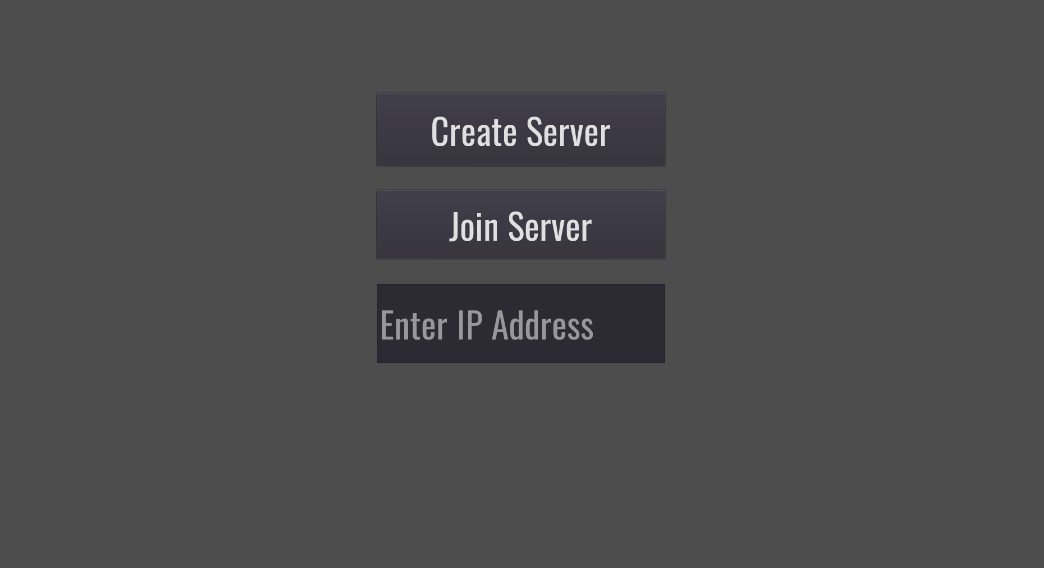
\includegraphics[width=.9\linewidth]{Images/prototype/prototype_net_menu.png}
    \caption{Menu startowe prototypu po wprowadzeniu systemu sieciowego}
    \label{fig:prototype_menu}
\end{figure}

Na interfejsie menu widoczne s� dwa przyciski. Przycisk ``Create Server'' powoduje rozpocz�cie gry jako host. Gra hostowana jest wtedy na adresie IP maszyny u�ytkownika. Przycisk ``Join Server'' powoduje rozpocz�cie gry na serwerze, kt�rego adres IP wpisany jest w pole tekstowe. W prototypie nie zosta�y zastosowane �adne techniki obrony przed wpisaniem niepoprawnego adresu IP ani pr�by po��czenia z nieistniej�cym serwerem.

Skrypt globalny \texttt{Network} jest odpowiedzialny za po��czenia sieciowe. Korzysta on z wysokopoziomowego interfejsu sieciowego Godota. 

Podczas uruchomienia gry ten skrypt pobiera adres IP maszyny. Nast�pnie ��czy si� z sygna�ami zwi�zanymi ze zmianami sieciowego stanu gry (Listing \ref{lst:signal_connecting_prototype}). 


\begin{lstlisting}[language=python,caption=Pod��czanie do najwa�niejszych sygna��w sieciowych, label=lst:signal_connecting_prototype ,basicstyle=\footnotesize\ttfamily]
get_tree().connect("connected_to_server", self, "_connected_to_server")
get_tree().connect("server_disconnected", self, "_server_disconnected")
get_tree().connect("network_peer_connected", self, "_player_connected")
get_tree().connect("network_peer_disconnected",self,"_player_disconnected")
\end{lstlisting}

Poni�ej zosta�y opisane sygna�y oraz przypisane do nich funkcje:
\begin{itemize}
    \item \texttt{connected\_to\_server} zostaje emitowany gdy gra po��czy si� z serwerem. Funkcja tworzy instancj� w�asnej postaci gracza.
    \item \texttt{server\_disconnected} zostaje emitowany gdy gra zostanie roz��czona z serwerem; W prototypie funkcja jedynie loguje wydarzenie.
    \item \texttt{network\_peer\_connected} zostaje emitowany gdy inny gracz zostaje pod��czony do gry. W sytuacji gdy gracz pierwszy raz pod��cza si� do serwera ten sygna� emitowany jest dla wszystkich graczy ju� na serwerze. Funkcja tworzy instancj� postaci nowo pod��czonego gracza.
    \item \texttt{network\_peer\_disconnected} zostaje emitowany gdy inny gracz od��cza si� od serwera. Funkcja usuwa posta� roz��czonego gracza.
\end{itemize}

Ponadto w skrypcie \texttt{Network} zdefiniowane s� funkcje \texttt{create\_server} i \texttt{join\_server} s�u��ce do, odpowiednio, stworzenia serwera i do��czenia do serwera. W tym celu wykorzystana zosta�a klasa \texttt{NetworkedMultiplayerENet}, implementuj�ca warstw� sieciow� korzystaj�c� z po��czenia UDP.


\begin{lstlisting}[language=python,caption=Funkcja inicjuj�ca serwer gry., label=lst:create_server_prototype ,basicstyle=\footnotesize\ttfamily]
func create_server() -> void:
  server = NetworkedMultiplayerENet.new()
  server.create_server(DEAFAULT_PORT, MAX_CLIENTS)
  get_tree().set_network_peer(server)
\end{lstlisting}
\begin{lstlisting}[language=python,caption=Funkcja ��cz�ca do serwera gry., label=lst:join_server_prototype ,basicstyle=\footnotesize\ttfamily]
func join_server() -> void:
  client = NetworkedMultiplayerENet.new()
  client.create_client(ip_address, DEAFAULT_PORT)
  get_tree().set_network_peer(client)
\end{lstlisting}

Skrypt \texttt{Global} sk�ada si� z metod u�atwiaj�cych instancjonowanie graczy. S� one wykorzystywane podczas rozpoczynania gry.

Do sceny gracza dodano w�z�y \texttt{Timer} - odliczaj�cy okres synchronizacji z serwerem i \texttt{Tween} - pozwalaj�cy p�ynnie przekszta�ca� w�a�ciwo�ci w�z�a. Do skryptu gracza dodano zmienne oznaczone s�owem kluczowym typu \texttt{puppet} - s� to warto�ci, kt�re b�d� synchronizowane przez sie�. Takie zmienne stworzono dla pozycji i rotacji gracza, rotacji wie�yczki oraz pr�dko�ci gracza. 

\texttt{Timer} ustawiony zosta� na okres 0.3 sekundy. Co taki okres wysy�a on sygna�, kt�ry wywo�uje funkcj� synchronizuj�c� warto�ci zmiennych puppet po sieci. W momencie ustawienia w ten spos�b pozycji jest ona interpolowana z wykorzystaniem w�z�a \texttt{Tween}. Jest to implementacja za�o�e� z sekcji \ref{sec:concept_prediction}. Posta� gracza wysy�a wtedy warto�� swoich rzeczywistych zmiennych. Awatar gracza w grze pozosta�ych graczy w procesie fizycznym zmienia r�wnie� rotacj� cia�a i wie�yczki. Je�eli \texttt{Tween} nie jest aktywny, posta� jest przemieszczana z pr�dko�ci� otrzyman� z sieci. Jest to implementacja predykcji klienckich, r�wnie� z sekcji \ref{sec:concept_prediction}.


\section{Wnioski}

Zgodnie z za�o�eniami, przygotowanie prototypu pozwoli�o zapozna� si� z zawi�o�ciami silnika Godot oraz zlokalizowa� przysz�e trudno�ci. 

Implementacja podstawowych mechanik nie b�dzie stanowi� wi�kszych trudno�ci. Zostan� one zaimplementowane w spos�b zbli�ony do tego z prototypu. Po��czenie sieciowe b�dzie stanowi�o najwi�ksze wyzwanie. Aby jego implementacja przebieg�a sprawnie niezb�dny b�dzie dok�adny projekt modelu danych oraz ich przep�ywu przez sie�. Jednak zastosowanie wysokopoziomowej warstwy sieciowej silnika Godot pozwoli znacznie upro�ci� ca�y system sieciowy.



\chapter{Projekt aplikacji}
\section{Interfejs u�ytkownika}
\section{Implementacja mechanik}
\section{System sieciowy}
\chapter{Implementacja}
\section{Interfejs użytkownika}
Z wykorzystaniem wbudowanych w Godot węzłów zbudowane zostały interfejsy zaprojektowane w sekcji \ref{sec:interface_design}. Problematyczne okazało się dostosowanie układu tak, aby przy zmianie rozmiaru okna elementy nie nachodziły na siebie. Dodatkowo, przy skalowaniu okna nie ma możliwości dynamicznego dostosowania wielkości czcionki do wielkości kontrolki w której się znajduje.  Było to szczególnym problemem podczas testowania oprogramowania, kiedy często należało uruchamiać kilka instancji na jednym ekranie. W domyślnym użytkowaniu gry taki problem nie powinien występować, ponieważ gra będzie rozgrywana na pełnym ekranie.

W celu ustawienia kontrolek w odpowiednich miejscach i w odpowiednich relacjach wykorzystane zostały węzły kontenerowe: \texttt{VBoxContainer}, \texttt{HBoxContainer} i \texttt{GridContainer}.

Innym problemem napotkanym podczas implementacji okazało się przełączanie scen. Problem był zauważalny między rundami, gdzie menu wyboru kart nie było wyświetlane mimo, że powinno było. Problemem okazał się być fakt, iż przełączenie sceny nie dzieje się od razu. Jest ono odsunięte w czasie na klatkę po wykonaniu całej funkcji. Dodatkowo zmiana sceny nie powoduje zakończenia funkcji. Doprowadziło to do sytuacji, w której scena była zmieniana wielokrotnie w jednym wykonaniu. Po odnalezieniu powodu takiego zachowania w dokumentacji rozwiązaniem było opuszczanie funkcji słowem kluczowym \texttt{return} po zamianie sceny.

HUD gracza podzielono na podelementy. Oddzielnie przygotowano scenę informacji własnych gracza, oddzielnie zaś scenę informacji innych graczy. Sceny te połączono z danymi na temat żywotności i liczby pocisków poszczególnych graczy przy pomocy sygnałów. Sceny z informacjami innych graczy tworzone i dodawane są do gry w momencie rozesłania sygnału rozpoczęcia rozgrywki. Pełna scena HUD dodana została do sceny gracza. Sprawia to, że jest ona stale dostępna w oknie gry, jednak w przypadku uruchomienia sceny menu, HUD jest przez nią zasłaniany.

W menu kart, same karty również zostały przygotowane jako oddzielne sceny. Pozwala to na łatwe generowanie widoku z różnymi kartami, wyglądającymi tak samo. Jako tło karty ustawiony został węzeł \texttt{TextureRect}. Umożliwia to w przyszłości przygotowanie różnorodnych grafik dla różnych kart. W aktualnej implementacji. Podjęte zostały również próby umieszczenia na karcie informacji na temat modyfikowanych atrybutów, jednak potencjalnie duża możliwa ich liczba doprowadziła do decyzji o ukryciu ich przed graczem.

\section{Postać gracza}
Model postaci został przygotowany w programie Blender (rys. \ref{fig:model}). Ze względu na prostsze wykonanie, sam model wykonano w stylu \emph{low poly} (ang. mało wielokątów). Przygotowane zostały również materiały: pokrywający lufę i gąsienice oraz dwa pokrywające karoserię i wieżyczkę. W grze materiały kolorowe zostają zmodyfikowane tak, aby ich kolorem bazowym był ten wybrany przez gracza (rys. \ref{fig:model_green}).

\begin{figure}
\centering
    \begin{subfigure}{.7\textwidth}
        \centering
        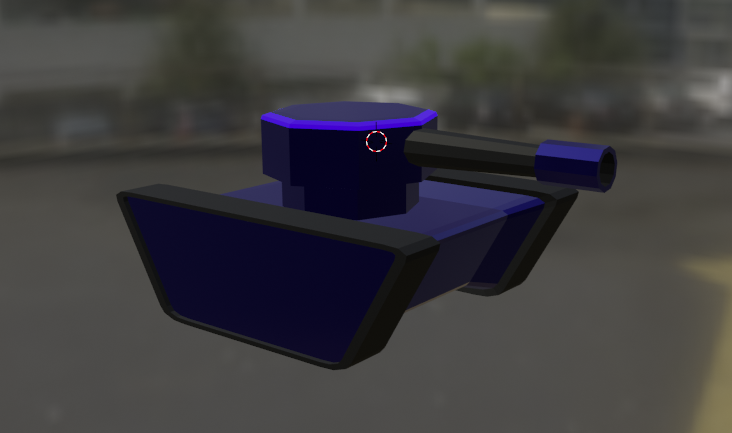
\includegraphics[width=.8\linewidth]{Images/development/model.png}
        \caption{Model w programie Blender.}
        \label{fig:model}
    \end{subfigure}
    
    \begin{subfigure}{.7\textwidth}
        \centering
        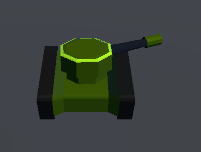
\includegraphics[width=.8\linewidth]{Images/development/model_green.png}
        \caption{Model o programowo zmienionych barwach.}
        \label{fig:model_green}
    \end{subfigure}
    \caption{Model czołgu.}
    \label{fig:both_models}
\end{figure}



\section{Implementacja mechanik}

\section{System sieciowy}

\section{Testy}

\section{Wyniki implementacji}


\chapter{Podsumowanie}

\section{Wnioski}
Aplikacja została w pełni zaimplementowana zgodnie z wymaganiami i koncepcją. Korzystanie z silnika Godot znacznie ułatwiło pracę nad wieloma aspektami gry. Wprowadzenie systemu sieciowego było o wiele prostszym zadaniem niż wyglądało. Mimo to w przypadku dalszego rozwoju warto byłoby dokładniej zaplanować działanie tego systemu. Szczególnie w przypadku znacznego rozrostu funkcjonalności gry niezbędne może okazać się zbudowanie kodu sieciowego od nowa tak, aby podział odpowiedzialności był oczywisty. W przygotowanej implementacji zdarza się, że podobne zachowanie aplikacji wywoływane jest z wielu powodów. 

Rozpoczęcie pracy od przygotowania koncepcji i prototypu pomogło głębiej zrozumieć działanie silnika Godot oraz jego interfejsów sieciowych. Błędem było jednak budowanie dalszych rozwiązań bezpośrednio na implementacji prototypu. Lepszym rozwiązaniem byłoby zbudowanie ostatecznej implementacji niezależnie, korzystając jedynie ze zdobytej wiedzy.

Język GDScript wykorzystany w projekcie jest prostym, czytelnym i bardzo łatwym w obsłudze narzędziem. Autor projektu odczuł jednak, że brak silnego typowania oraz nietypowa implementacja obiektowego paradygmatu programowania opóźniały pracę i wprowadzały błędy, których możnaby uniknąć w innych językach. Ponadto korzystanie z innych języków programowania wiązałoby się z możliwościom korzystania z ich, o wiele bogatszej dokumentacji i dokładniejszej oraz materiałów edukacyjnych dostępnych w Internecie.

\section{Znane problemy}
Istnieje znany problem którego dotychczas nie udało się rozwiązać. W czasie rozgrywki co jakiś czas pojawiają się błędy kamery, obraca się ona i przesuwa w chaotyczny sposób. Możliwe, że jest to związane z aktualizacjami pozycji spowodowanymi opóźnieniem połączenia internetowego, ciężko jest jednak sprawdzić tego typu błędy. 

\section{Dalszy rozwój projektu}
Istnieje wiele możliwości dalszego rozwoju projektu. Podzielić je można na dwie główne grupy. Rozwój ,,techniczny'' jest związany z poprawą jakości technologicznej części projektu oraz dodaniem dodatkowych funkcjonalności. Rozwój ,,kreatywny'' wiąże się z poszerzeniem sfery \emph{game designu} oraz audiowizualnej.

\subsection{Warstwa techniczna}
Wśród możliwości technicznych większość ma związek z usprawnieniem kodu sieciowego. Jednym z możliwych usprawnień byłoby stworzenie dedykowanej aplikacji serwerowej, tj. takiej bez warstwy wizualnej, uruchamianej na przykład jako polecenie terminala. Taka aplikacja nie mogłaby być związana z żadną postacią gracza. Stworzenie takiej wersji aplikacji jest możliwe z wykorzystaniem Godota. Może to być oddzielna aplikacja lub inaczej uruchamiana modyfikacja przygotowanego projektu.

Alternatywą mogłoby być wprowadzenie obsługi zewnętrznej usługi serwerów. Przykładem gotowego rozwiązania sieciowego którego obsługę możnaby wprowadzić są serwery Steam. Istnieje rozszerzenie Godota pozwalające na wprowadzenie ich obsługi. Wymagałoby to jednak najpewniej zupełnej przebudowy kodu sieciowego.

Kolejnym aspektem technicznym możliwym do dodania jest wprowadzenie obsługi kontrolerów oraz własne mapowanie wejść przez gracza. Oba z tych rozwiązań są wspierane przez silnik, istnieje więc możliwość prostego wprowadzenia takich rozszerzeń.

Aktualnie aplikacja obsługiwana jest jedynie w języku angielskim. Wartym rozważenia rozszerzeniem mogłoby być wprowadzenie tłumaczeń na inne języki. Wprowadzanie tłumaczeń jest wspierane przez Godot.

W grze rozwinięta została w pewnym stopniu warstwa wizualna, wiele mogłoby jednak dodać również wprowadzenie obsługi dźwięków takich jak odgłosy czołgów graczy, strzałów czy eksplozji. Ponadto, warstwa wizualna mogłaby zostać rozbudowana o animacje. Wprowadzenie cieni i realistycznych odbić w obiektach metalicznych zostało wypróbowane, jednak wygląd takich rozwiązań był niezadowalający.

Istotnym elementem po dodaniu powyższych rozszerzeń jest wprowadzenie menu ustawień, w którym gracz mógłby zmieniać aspekty działania aplikacji. Ponadto do gry powinno zostać dodane menu pauzy, w którym gracz mógłby zobaczyć listę aktualnie posiadanych kart.

\subsection{Warstwa kreatywna}
Ciekawym rozszerzeniem i urozmaiceniem gry jest dodanie dodatkowych trybów rozgrywki. W innych trybach gracze dostawaliby punkty za osiąganie innych celów, mogliby również łączyć się w zespoły i współpracować.

Oczywistym dodatkiem do gry jest również poszerzenie bazy dostępnych kart. Korzystając z aktualnie dostępnych systemów możliwe jest stworzenie wielu ciekawych kombinacji. Dodatkowym aspektem może być również dodanie kolejnej akcji, na przykład uruchamianej drugim przyciskiem myszy. Byłaby ona uruchamiana w punkcie, w którym znajduje się gracz. Taka mechanika również korzystałaby z komend.

Innym sposobem na urozmaicenie gry jest rozwinięcie warstwy wizualnej. Jedną z możliwości jest tu wprowadzenie dodatkowych poziomów. Każda runda mogłaby wtedy rozgrywać się na losowym poziomie o różnych charakterystykach. Dodanie do poziomów zagrożeń środowiskowych również mogłoby rozszerzyć możliwości tworzenia kolejnych poziomów.

Kolejnym artystycznym aspektem możliwym do rozwinięcia jest wprowadzenie grafik do menu, ekranów i jako ikonę gry. Ponadto wprowadzenie kolejnych możliwości personalizacji modeli również może urozmaicić rozgrywkę.

% % !TEX encoding = UTF-8 Unicode 
% !TEX root = praca.tex

\chapter{Tytuł rozdziału I}

W książce \cite{docker_compose_reference} \dots



\section{Rysunki}

\begin{figure}
\centering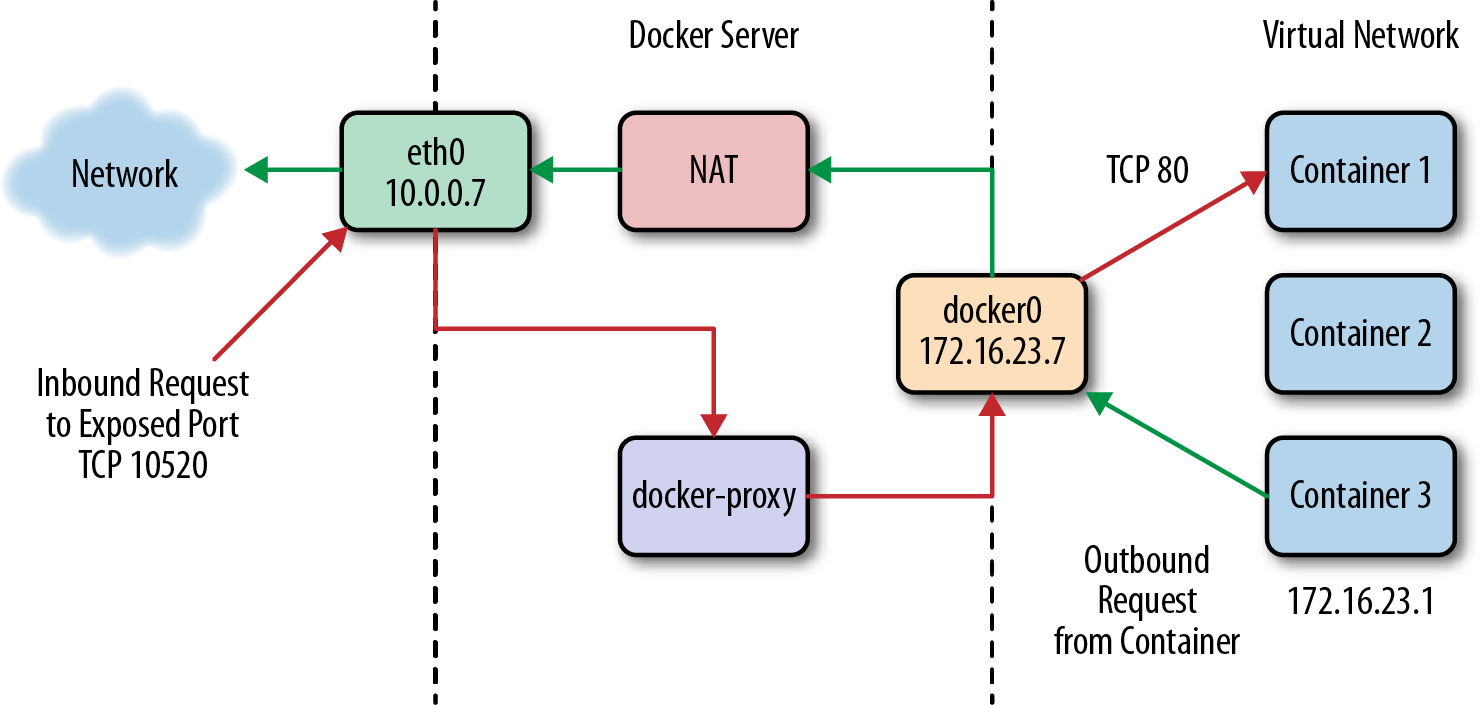
\includegraphics[width=.6\textwidth]{img/swarm-network}
\caption{Sieć dokera \cite{docker_compose_reference}}  \label{rys:network}
\end{figure}

Na rysunku \ref{rys:network} \dots


\subsection{Dwa rysunki obok siebie}

\begin{figure}[h] 
	\centering
	\begin{minipage}[b]{0.45\textwidth}
		\centering
\includegraphics[width=0.9\textwidth]{img/kotek} % left figure
		\caption{Lewy rysunek}\label{fig:lewy}
	\end{minipage}
	\begin{minipage}[b]{0.45\textwidth}
		\centering
		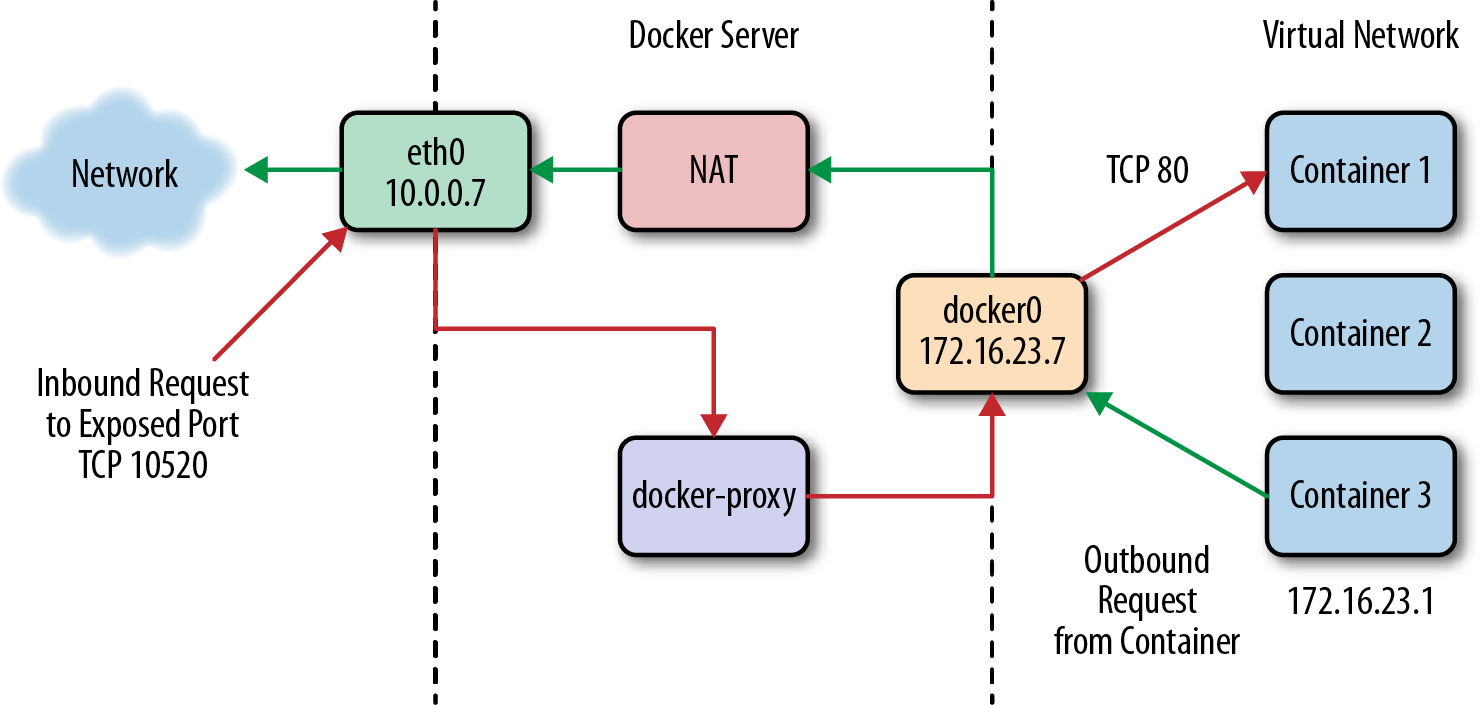
\includegraphics[width=0.9\textwidth]{img/swarm-network} % right figure
		\caption{Prawy rysunek}\label{fig:prawy}
	\end{minipage}
\end{figure}

Na rysunkach \ref{fig:lewy} i \ref{fig:prawy} \dots


\section{Tabele}

W tabeli \ref{table:table1} \dots

\begin{table}
\centering\caption{Tytuł tabeli (patrz dodatek~\ref{app1}) \label{table:table1}}
\begin{tabular}{|l|l|l|}% table alignment -> l c r - left, center, right
\hline
Pierwszy & Drugi & Trzeci \\
\hline
Pierwszy & Drugi & Trzeci \\
\hline
\end{tabular}
\end{table}

\subsection{Równania}

\begin{equation}
\sum_{i=1}^{\infty}a_i
\label{eq:myEquation}
\end{equation}

W równaniu \ref{eq:myEquation} \dots

\section{Listingi}

Na listingu \ref{listing:myListing} \dots

% replace {c} with the appropriate language
\begin{listing}
\begin{minted}{c}  
int main()
{
   int a=2*3;
   printf("**Ala ma kota\n**");
   while(!I2C_CheckEvent(I2C1, I2C_EVENT_MASTER_MODE_SELECT)); /* EV5 */
   return 0;
}
\end{minted}
\caption{Język C} \label{listing:myListing}
\end{listing}


% /

% % !TEX encoding = UTF-8 Unicode 
% !TEX root = praca.tex

\chapter*{Podsumowanie}

\lipsum[17]



% Bibliography
\bibliographystyle{unsrt}
\bibliography{bibliography}

% Lists of figures, listings, tables
\listoffigures
% \listoflistings
\listoftables

% Appendices - comment out if not applicable
% \appendixpage
% \appendix
% \chapter{Dodatek 1}\label{app1}

\lipsum[20]

\end{document}
